\section{Expected Benefits}
\label{chap:improvement:benefits}

\mnote{Benefits overview}
We expect several benefits from the \commonalities approach in comparison to defining ordinary networks of transformations.
First, we claim to achieve better \emph{comprehensibility} by making common concept explicit rather than implicitly encoding them in consistency relations.
Second, we mitigate trade-offs between specific quality properties, in particular correctness and reusability, of the defined transformation network.
Finally, it promises to reduce the specification effort at least in specific scenarios.
While the improvement in comprehensibility is only a claim, we discuss the benefits of mitigating trade-offs and reducing specification effort in the following.


\subsection{Improving Correctness and Reusability}
\label{chap:improvement:benefits:properties}

\mnote{Correctness and reusability}
We have discussed the benefits of the \commonalities approach regarding correctness guarantees in \autoref{chap:improvement:commonalities:tree}.
This results from a transformation network defined with the \commonalities approach being intended to induce a tree topology.
At the same time, a network defined by \commonalities also improves reusability, although the network forms a tree and reusability is actually a benefit of dense graphs as discussed in \autoref{chap:classification:topologies:effects}.

\begin{figure}
    \centering
    \begin{minipage}[b]{0.49\columnwidth}
        \centering
        \newcommand{\hmmdistance}{3.6em}
\newcommand{\vmmdistance}{2.4em}

\begin{tikzpicture}[
    mm/.style={schematic metamodel},
]

\node[mm] (full_left) {};
\node[mm, above right=\vmmdistance and \hmmdistance of full_left.center, anchor=center] (full_top) {};
\node[mm, below right=\vmmdistance and \hmmdistance of full_left.center, anchor=center] (full_bottom) {};
\node[mm, right=2*\hmmdistance of full_left.center, anchor=center] (full_right) {};
\node[mm, below left=\vmmdistance and \hmmdistance of full_left.center, anchor=center] (full_bottomleft) {};

\draw[transformation] (full_left) -- (full_top);
\draw[transformation] (full_left) -- (full_right);
\draw[transformation] (full_left) -- (full_bottom);
\draw[transformation] (full_top) -- (full_right);
\draw[transformation] (full_top) -- (full_bottom);
\draw[transformation] (full_right) -- (full_bottom);
\draw[transformation] (full_left) -- (full_bottomleft);
\draw[transformation] (full_bottom) -- (full_bottomleft);
\draw[transformation] (full_top) to[bend right=30] (full_bottomleft);
\draw[transformation] (full_bottomleft) .. controls ++(1*\hmmdistance, -0.8*\vmmdistance) and ([yshift=-1.5*\vmmdistance]full_right.south) .. (full_right);

\end{tikzpicture}
        \subcaption{Complete Graph}
        \label{fig:improvement:topologies:complete}
    \end{minipage}
    \hfill
    \begin{minipage}[b]{0.49\columnwidth}
        \centering
        \newcommand{\hmmdistance}{3.6em}
\newcommand{\vmmdistance}{2.4em}

\begin{tikzpicture}[
    conceptmm/.style={schematic conceptmetamodel},
    concretemm/.style={schematic metamodel},
]

\node[conceptmm, right=4*\hmmdistance of full_left.center, anchor=center] (tree_left) {};
\node[conceptmm, above right=\vmmdistance and \hmmdistance of tree_left.center, anchor=center] (tree_top) {};
\node[concretemm, below right=\vmmdistance and \hmmdistance of tree_left.center, anchor=center] (tree_bottom) {};
\node[concretemm, right=2*\hmmdistance of tree_left.center, anchor=center] (tree_right) {};
\node[concretemm, below left=\vmmdistance and \hmmdistance of tree_left.center, anchor=center] (tree_bottomleft) {};

\draw[transformation] (tree_left) -- (tree_top);
\draw[transformation] (tree_left) -- (tree_bottom);
\draw[transformation] (tree_left) -- (tree_bottomleft);
\draw[transformation] (tree_top) -- (tree_right);

\end{tikzpicture}
        \vspace{1em}
        \subcaption{\commonalities Tree}
        \label{fig:improvement:topologies:tree}
    \end{minipage}
    \caption[Benefit of \commonalities regarding quality trade-offs]{Complete graphs as an extreme of transformation network topologies in comparison to the tree topology of a \commonalities specification. Nodes depict metamodels and edges depict transformations. In a \commonalities specification, leaves represent \concretemetamodels whereas inner nodes represent \conceptmetamodels. Adapted from~\owncite[Fig. 4]{klare2019models}.}
    \label{fig:improvement:topologies}
\end{figure}

\mnote{Extreme topologies}
\autoref{fig:improvement:topologies} depicts the topology extremes of complete graphs and trees.
In the tree topology of a \commonalities specification, the \concretemetamodels are represented by leaves of the tree, whereas the inner nodes represent \conceptmetamodels.
This depiction is reduced to metamodels rather than \metaclasses and \commonalities, as discussed in \autoref{chap:improvement:commonalities:tree} for the tree structure, but would be the same if considered at the level of \metaclasses.

\mnote{Reusability in trees}
In \autoref{chap:classification:topologies:effects}, we have discussed that reusability is improved in transformation networks inducing a dense or even complete graph, as a transformation exists for each metamodel pair and thus the transformations for any subset of the metamodels can be reused in other transformation networks relating a different set of metamodels.
Having a tree topology, only subtrees can be reused, as otherwise consistency between some of the metamodels cannot be preserved because it was expressed transitively via transformations across metamodels that are not part of the subset to be reused.

\mnote{Reusability in \commonalities}
This is, however, different for a network defined with the \commonalities approach.
Although it forms a tree, the \concretemetamodels to be reused in other networks are only leaves of that tree.
Any subset of them can be reused without loosing transformations that preserve consistency between them by also reusing all \conceptmetamodels on each path between two of the \concretemetamodels to reuse.
Since \conceptmetamodels and their instances only represent auxiliary artifacts for describing consistency relations and their preservation, it is not a drawback that they have to be reused.

\mnote{Trade-off mitigation}
For these reasons, defining consistency with the \commonalities approach has the same benefits regarding correctness (and also other maintainability properties as discussed in \autoref{chap:classification:topologies:effects}) as defining a transformation network with tree topology, but at the same it improves reusability by allowing any subset of the \concretemetamodels and the specification of consistency between them to be reused.
The central limitation of the approach is regarding completeness, since the manifestation relations between \metaclasses and \commonalities must induce a specific tree structure, namely a consistency relation tree according to \autoref{def:relationtree}, to actually provide the benefits regarding correctness.
It is part of our evaluation in \autoref{chap:commonalities_evaluation} to validate the achievability of that property in practical scenarios.

% \begin{figure}
%     \centering
%     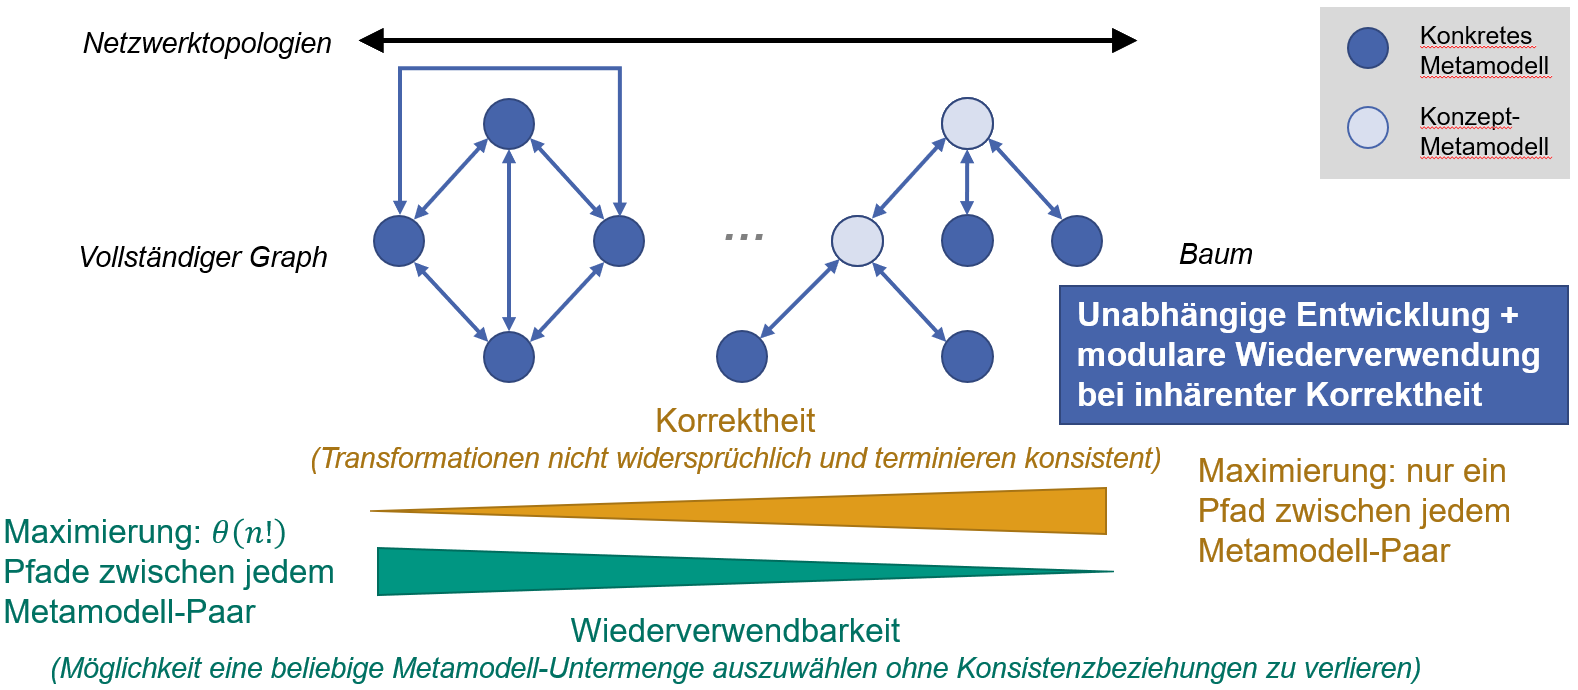
\includegraphics[width=\textwidth]{figures/quality/improvement/benefit_tradeoff.png}
%     \caption[Benefit of \commonalities regarding quality trade-offs]{Reduction of trade-off between quality properties using the \commonalities approach by ensuring correctness through a tree topology and achieving reusability by \concretemetamodels only being leaves.}
%     \label{fig:improvement:benefit_tradeoff}
% \end{figure}


\subsection{Reducing Specification Effort}
\label{chap:improvement:benefits:specification_effort}

\mnote{Redundancies in consistency relations}
While the mitigation of the trade-off between correctness and reusability of a transformation network through the use of the \commonalities approach represents its major benefit, it can also reduce specification effort.
This is achieved by the fact that each consistency relation must, in the best case, only be defined once, whereas in a transformation network inducing a dense or even a complete graph, there need to be redundant representations of the same relations if arbitrary parts of the network are supposed to be reusable.

\begin{figure}
    \centering
    \newcommand{\classwidth}{5em}
\newcommand{\hdistance}{11em}
\newcommand{\innerhdistance}{10em}
\newcommand{\labeldistance}{1em}
\newcommand{\mmborder}{1em}


\begin{tikzpicture}[
    manifests relation label/.style={stereotype, above, sloped}
]

\pgfdeclarelayer{bg}
\pgfsetlayers{bg,main}

\umlclassvarwidth{network_java_class}{}{Class}{
    name\\
    packageName
}{\classwidth}

\umlclassvarwidth[, right=\hdistance of network_java_class.north, anchor=north]{network_uml_class}{}{Class}{
    name
}{\classwidth}
\umlclassvarwidth[, right=\innerhdistance of network_uml_class.north, anchor=north]{network_uml_package}{}{Package}{
    name
}{\classwidth}

\umlclassvarwidth[, below right=0.5*\hdistance and \hdistance of network_java_class.north, anchor=north]{network_c_class}{}{Class}{
    name\\
    namespace
}{\classwidth}

\umlcomposition{(network_uml_package) -- node[uml role end, pos=1, above right] {classes} node[uml cardinality end, pos=1, below right] {*} (network_uml_class.east|-network_uml_package.west)}

\node[mmlabel, above=\labeldistance of network_java_class.north, anchor=center] (network_java_label) {Java};
\node[mmlabel, anchor=center] (network_uml_label) at ([yshift=\labeldistance]$(network_uml_class.north)!0.5!(network_uml_package.north)$) {\acrshort{UML}};
\node[mmlabel, below=\labeldistance of network_c_class.south, anchor=center] (network_c_label) {\cplusplus};

\begin{pgfonlayer}{bg}
    \node[mmbg, fit=(network_java_class)(network_java_label.center), inner sep=\mmborder] (network_java) {};
    \node[mmbg, fit=(network_uml_class)(network_uml_package)(network_uml_label.center), inner sep=\mmborder] (network_uml) {};
    \node[mmbg, fit=(network_c_class)(network_c_label.center), inner sep=\mmborder] (network_c) {};
\end{pgfonlayer}

\draw[transformation] (network_java_class.east|-network_uml_class.west) -- node[stereotype, above] {«transforms»} (network_uml_class);
\draw[transformation] (network_java_class.south) |- node[stereotype, above, pos=0.75] {«transforms»} (network_c_class.west);
\draw[transformation] (network_uml_class) -- node[stereotype, right] {«transforms»} (network_c_class);



\umlclassvarwidth[, below right=1.45*\hdistance and \hdistance of network_java_class.north, anchor=north]{comm_oo_class}{}{Class}{
    name
}{\classwidth}

\umlclassvarwidth[, right=\innerhdistance of comm_oo_class.north, anchor=north]{comm_oo_package}{}{Package}{
    name
}{\classwidth}

\umlcomposition{(comm_oo_package) -- node[uml role end, pos=1, above right] {classes} node[uml cardinality end, pos=1, below right] {*} (comm_oo_class.east|-comm_oo_package.west)}

\umlclassvarwidth[, below left=0.65*\hdistance and \hdistance of comm_oo_class.north, anchor=north]{comm_java_class}{}{Class}{
    name\\
    packageName
}{\classwidth}

\umlclassvarwidth[, right=\hdistance of comm_java_class.north, anchor=north]{comm_c_class}{}{Class}{
    name\\
    namespace
}{\classwidth}

\umlclassvarwidth[, right=\hdistance of comm_c_class.north, anchor=north]{comm_uml_package}{}{Package}{
    name
}{\classwidth}

\umlclassvarwidth[, below=0.5*\innerhdistance of comm_uml_package.north, anchor=north]{comm_uml_class}{}{Class}{
    name
}{\classwidth}

\umlcomposition{(comm_uml_package) -- node[uml role end, pos=1, above right] {classes} node[uml cardinality end, pos=1, above left] {*} (comm_uml_class)}

\coordinate (comm_oo_label_coordinate) at ($(comm_oo_class.north)!0.5!(comm_oo_package.north)$);
\node[mmlabel, above=\labeldistance of comm_oo_label_coordinate, anchor=center] (comm_oo_label) {Object-oriented Design};
\node[mmlabel, below=\labeldistance of comm_java_class.south, anchor=center] (comm_java_label) {Java};
\node[mmlabel, below=\labeldistance of comm_c_class.south, anchor=center] (comm_c_label) {\cplusplus};
\node[mmlabel, below=\labeldistance of comm_uml_class.south, anchor=center] (comm_uml_label) {\acrshort{UML}};

\begin{pgfonlayer}{bg}
    \node[conceptmmbg, fit=(comm_oo_class)(comm_oo_package)(comm_oo_label.center), inner sep=\mmborder] (comm_java) {};
    \node[mmbg, fit=(comm_java_class)(comm_java_label.center), inner sep=\mmborder] (comm_java) {};
    \node[mmbg, fit=(comm_c_class)(comm_c_label.center), inner sep=\mmborder] (comm_c) {};
    \node[mmbg, fit=(comm_uml_class)(comm_uml_package)(comm_uml_label.center), inner sep=\mmborder] (comm_uml) {};
\end{pgfonlayer}

\draw[manifests relation] (comm_oo_class) -- node[manifests relation label] {\manifestslabel} (comm_java_class);
\draw[manifests relation] (comm_oo_class) -- node[manifests relation label] {\manifestslabel} (comm_c_class);
\draw[manifests relation] (comm_oo_class) -- node[manifests relation label] {\manifestslabel} (comm_uml_class);
\draw[manifests relation] (comm_oo_package) -- node[manifests relation label] {\manifestslabel} (comm_uml_package);


\node[above=3*\labeldistance of network_uml_class.north, anchor=center, font=\small\bfseries] {Transformation Network};
\node[above=3*\labeldistance of comm_oo_class.north, anchor=center, font=\small\bfseries] {\Commonalities Specification};

\end{tikzpicture}
    %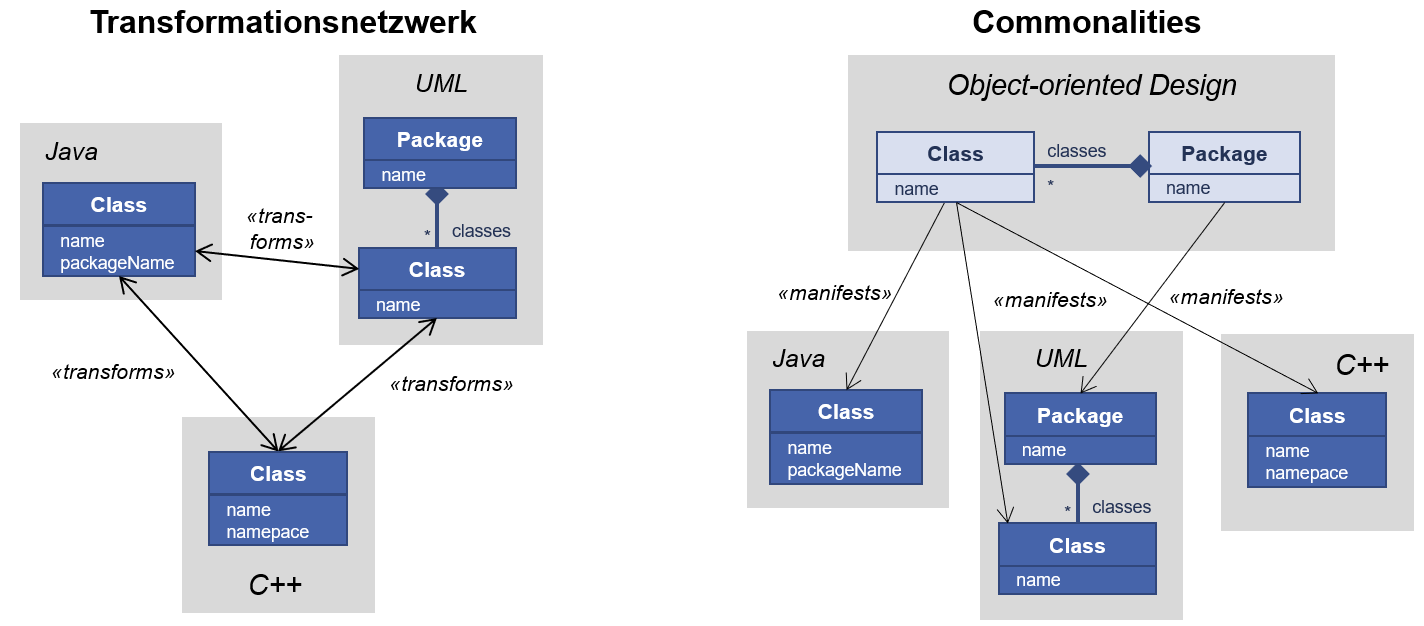
\includegraphics[width=\textwidth]{figures/quality/improvement/benefit_specification_effort.png}
    \caption[Benefit of \commonalities regarding specification effort]{Example for the number of defined relations with ordinary transformation networks and the usage of \conceptmetamodels with the \commonalities approach.}
    \label{fig:improvement:benefit_specification_effort}
\end{figure}

\mnote{Specification example}
\autoref{fig:improvement:benefit_specification_effort} depicts an the extension of the introductory example given in \autoref{fig:improvement:running_example}, in which in addition to classes in the \gls{UML} and Java a representation in \cplusplus is added.
In case of a transformation network, the relation between \cplusplus and both Java and the \gls{UML} needs to be defined.
Using the \commonalities approach, only an additional manifestation relation to the concepts already defined in the object-oriented design \conceptmetamodels has to be specified.
In general, if $n$ metamodels share common concepts, adding an $n$-$1$-th metamodel requires $n$ transformations to be defined in ordinary networks, whereas the \commonalities approach, in the best case, only requires one addition manifestation relation to be defined.

\mnote{The average case}
The best case is, however, only achieved if the \conceptmetamodel already contains all information shared between the \concretemetamodel to be added and the ones for which the manifestation of the \commonalities in the \conceptmetamodel is already defined.
This is due to the already discussed fact that, informally speaking, the \conceptmetamodel needs to represent the union of all pairwise intersections of the \concretemetamodels.
Thus, it will usually be necessary to also extend or adapt the \conceptmetamodel and define or modify manifestations in the other \concretemetamodels as well.
For this scenario, a language that combines the specification of each \commonality with its manifestation relations, as we propose in \autoref{chap:language}, provides further benefits, as a modification or extension of a \commonality can be performed along with adaptations of the existing manifestation relations at one place.

\mnote{Initial effort}
In addition, applying the \commonalities approach may produce higher initial effort for the first consistency relations.
For two metamodels to keep consistent, one \conceptmetamodel and two manifestation relations have to be defined instead of only a single transformation in case of directly relating the two metamodels.
This initial effort amortizes only if enough further \concretemetamodels are kept consistent via the same \conceptmetamodel.

\mnote{Initial effort reduction}
The initial specification effort can, however, also be reduced by providing a specific language to define \commonalities that combines the definition of manifestation relations with the definition of its \commonality, such that the specification becomes nearly as concise as it would be if defined as a direct consistency relation between two metamodels.
We propose such a language in \autoref{chap:language} and discuss this benefit in \autoref{chap:language:commonalities:benefits}.
